\subsection{HTTP Interface}
This interface will be the library used for the server that will direct the incoming request to the controllers via a HTTP/TCP socket.

\begin{figure}[h!]
	\centering
 	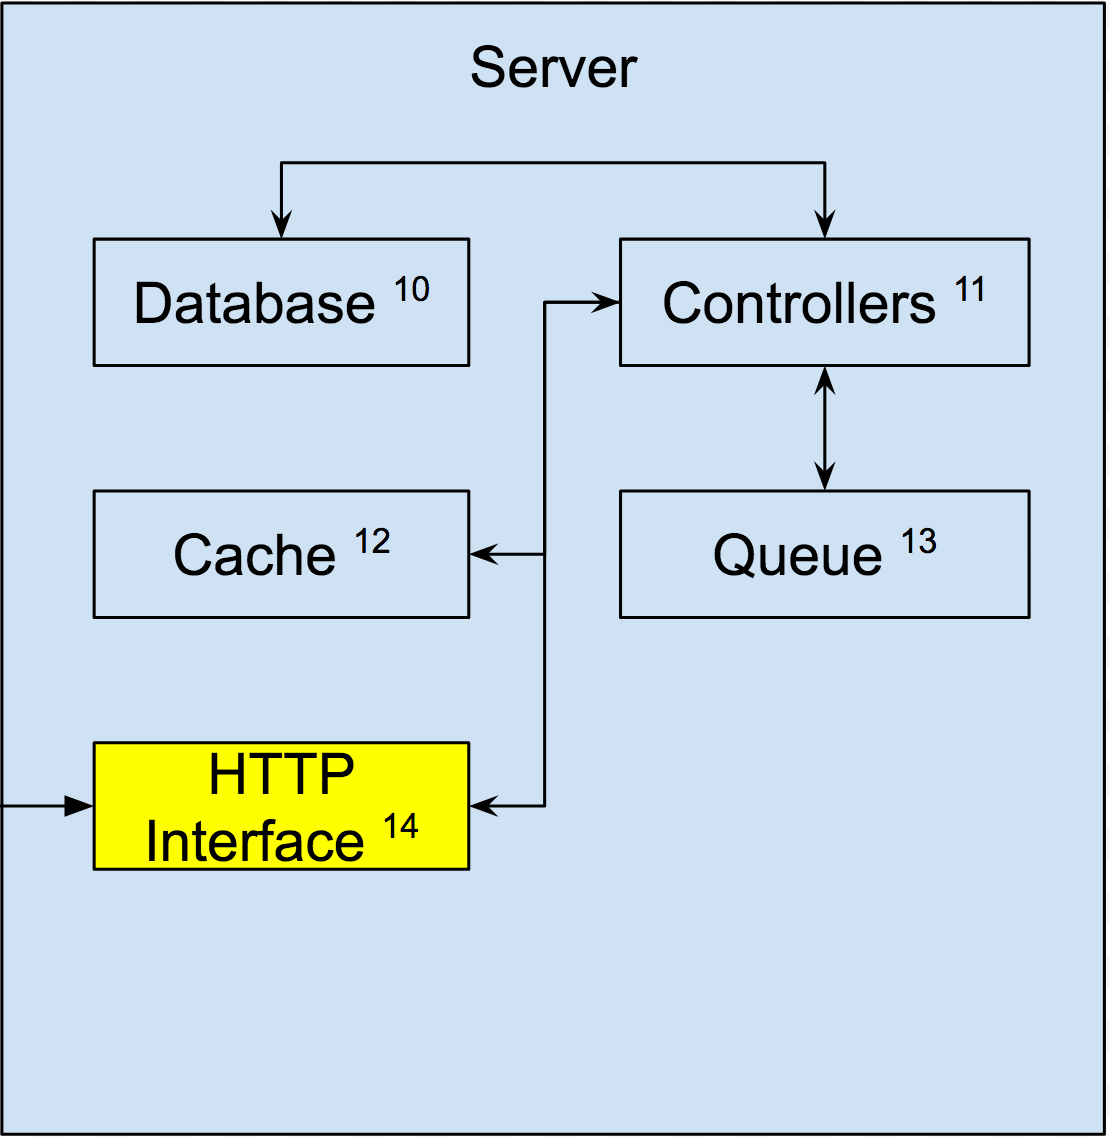
\includegraphics[width=0.60\textwidth]{images/server/server_http_interface.png}
 	\caption{Server-side HTTP Interface subsystem}
\end{figure}

\subsubsection{Assumptions}
N/A

\subsubsection{Responsibilities}
The responsibility of the HTTP interface will include receiving HTTP requests via a chosen open source library, which will request a resource from the controller subsystem. This interface will also make use of Go's built in http package, which will make requests on to the other third party services.

\subsubsection{Subsystem Interfaces}
\begin {table}[H]
\caption {Server-side HTTP Interface interfaces} 
\begin{center}
    \begin{tabular}{ | p{1cm} | p{6cm} | p{3cm} | p{3cm} |}
    \hline
    ID & Description & Inputs & Outputs \\ \hline
    \#01 & Request for login & \pbox{3cm}{JSON containing email and password} & \pbox{3cm}{JSON response containing either users info or an error}  \\ \hline
    \end{tabular}
\end{center}
\end{table}

\newpage
